\documentclass{beamer}
\usetheme{Amsterdam}
\setbeamertemplate{footline}{}
\logo{
\includegraphics[height=0.9cm]{HUG_logo.png}\hspace{15pt}}
\newcommand{\nologo}{\setbeamertemplate{logo}{}} % command to set the logo to nothing

\renewcommand{\baselinestretch}{1.15} % Line spacing
\usepackage{ragged2e} % Allign text, justify
\justifying
\setbeamertemplate{navigation symbols}{}
\usepackage{booktabs} % Table style
\usepackage{tabularx}
\usepackage{longtable}
\usepackage{graphicx}

\usepackage{etoolbox} % for joining title

\usepackage[style=authortitle,backend=biber]{biblatex}

\makeatletter
\patchcmd\beamer@@tmpl@frametitle{\insertframetitle}{\insertframetitle}{}{}
\makeatother

\usepackage[most]{tcolorbox}

\newtcolorbox{mysidebyside}[1][]{
    notitle, sidebyside,
    sidebyside align=center seam,
    halign=center,
    lefthand width=.1\textwidth,
    #1
}

\title{Arm-level Alterations in Cancer}
\author{CHASKAR Prasad, 
CHRISTINAT Yann and Dr. TSANTOULIS Petros}

\begin{document}

{
\begin{frame}
  \titlepage
\end{frame}
}


\section{Literature Review}

		\subsection{}
		
			\begin{frame}{}
			\begin{itemize}
						\pause
						\item Somatic copy number alterations (SCNA) are frequent genetic events that promote tumor initiation and progression.
						\pause
						\item SCNA comprise genetic losses or gains of varying size \footcite {Feuk2006}.
						\pause
						\item Focal SCNAs and Arm-level SCNAs.
			\end{itemize}
			\end{frame}

                \subsection{Focal SCNAs and Arm-level SCNAs}

               \begin{frame}
\begin{figure}
\centering
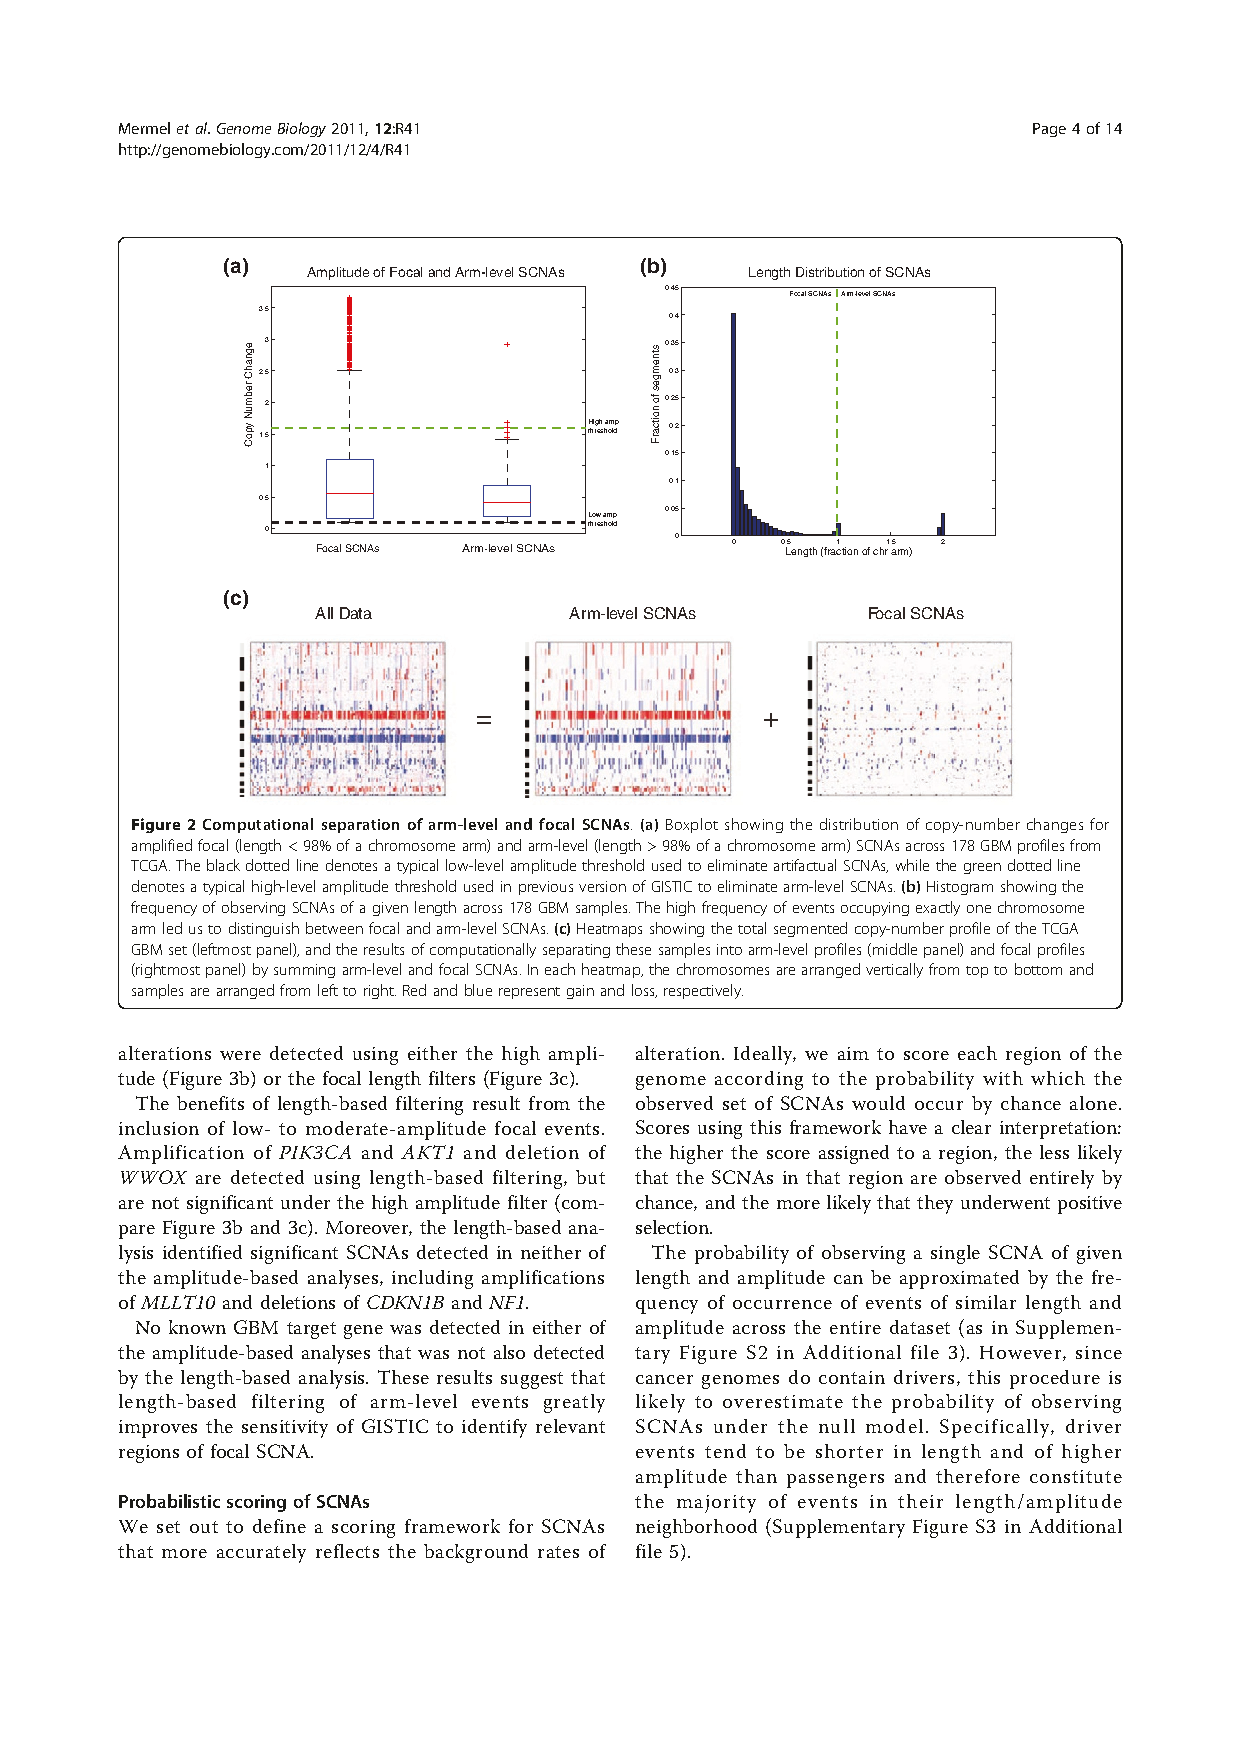
\includegraphics[width=0.9\textwidth, clip,trim=100 560 100 115]{/home/prasad/HUG/Presentation/Oncoscan/amplitue_length.pdf}
\caption{Separation of arm-level and focal SCNA \footcite {Mermel2011}}
\label{fig:stream}
\end{figure}
               \end{frame}

\section{Objectives}
		
			\begin{frame}{}
				\begin{flushleft}
			\begin{enumerate}
				\item Precise definition of an arm-level alteration
				\pause
				\begin{itemize}								
					\item Percentage of arm to be considered as ``arm-level''?
					\item Contiguity required?
					\item Use of smoothing function?
				\end{itemize}
				\pause
					\item Develop and validate tool for the prediction of arm-level alterations and focal alterations
			\end{enumerate}
				\end{flushleft}
			\end{frame}

\section{Approach}
%				\subsection{Inputs}
%				
%				\begin{frame}
%				\begin{enumerate}
%				\item Affymetrix OncoScan CNV Plus Assay
%				\pause
%				\item Enables the detection of relevant copy number variations (CNVs)
%				\begin{itemize}
%				\item Gain: 1-2 copies extra
%				\item Amplification: 5 and more copies
%				\item Loss: 1 copy loss or homozygous loss (2 copies lost)
%				\item LOH: 2 copies but loss of heterozygosity  
%				\end{itemize}
%				\end{enumerate}				 
%				\end{frame}
				
				\subsection{Oncoscan}
				
				\begin{frame}
				 \begin{figure}
				\centering
				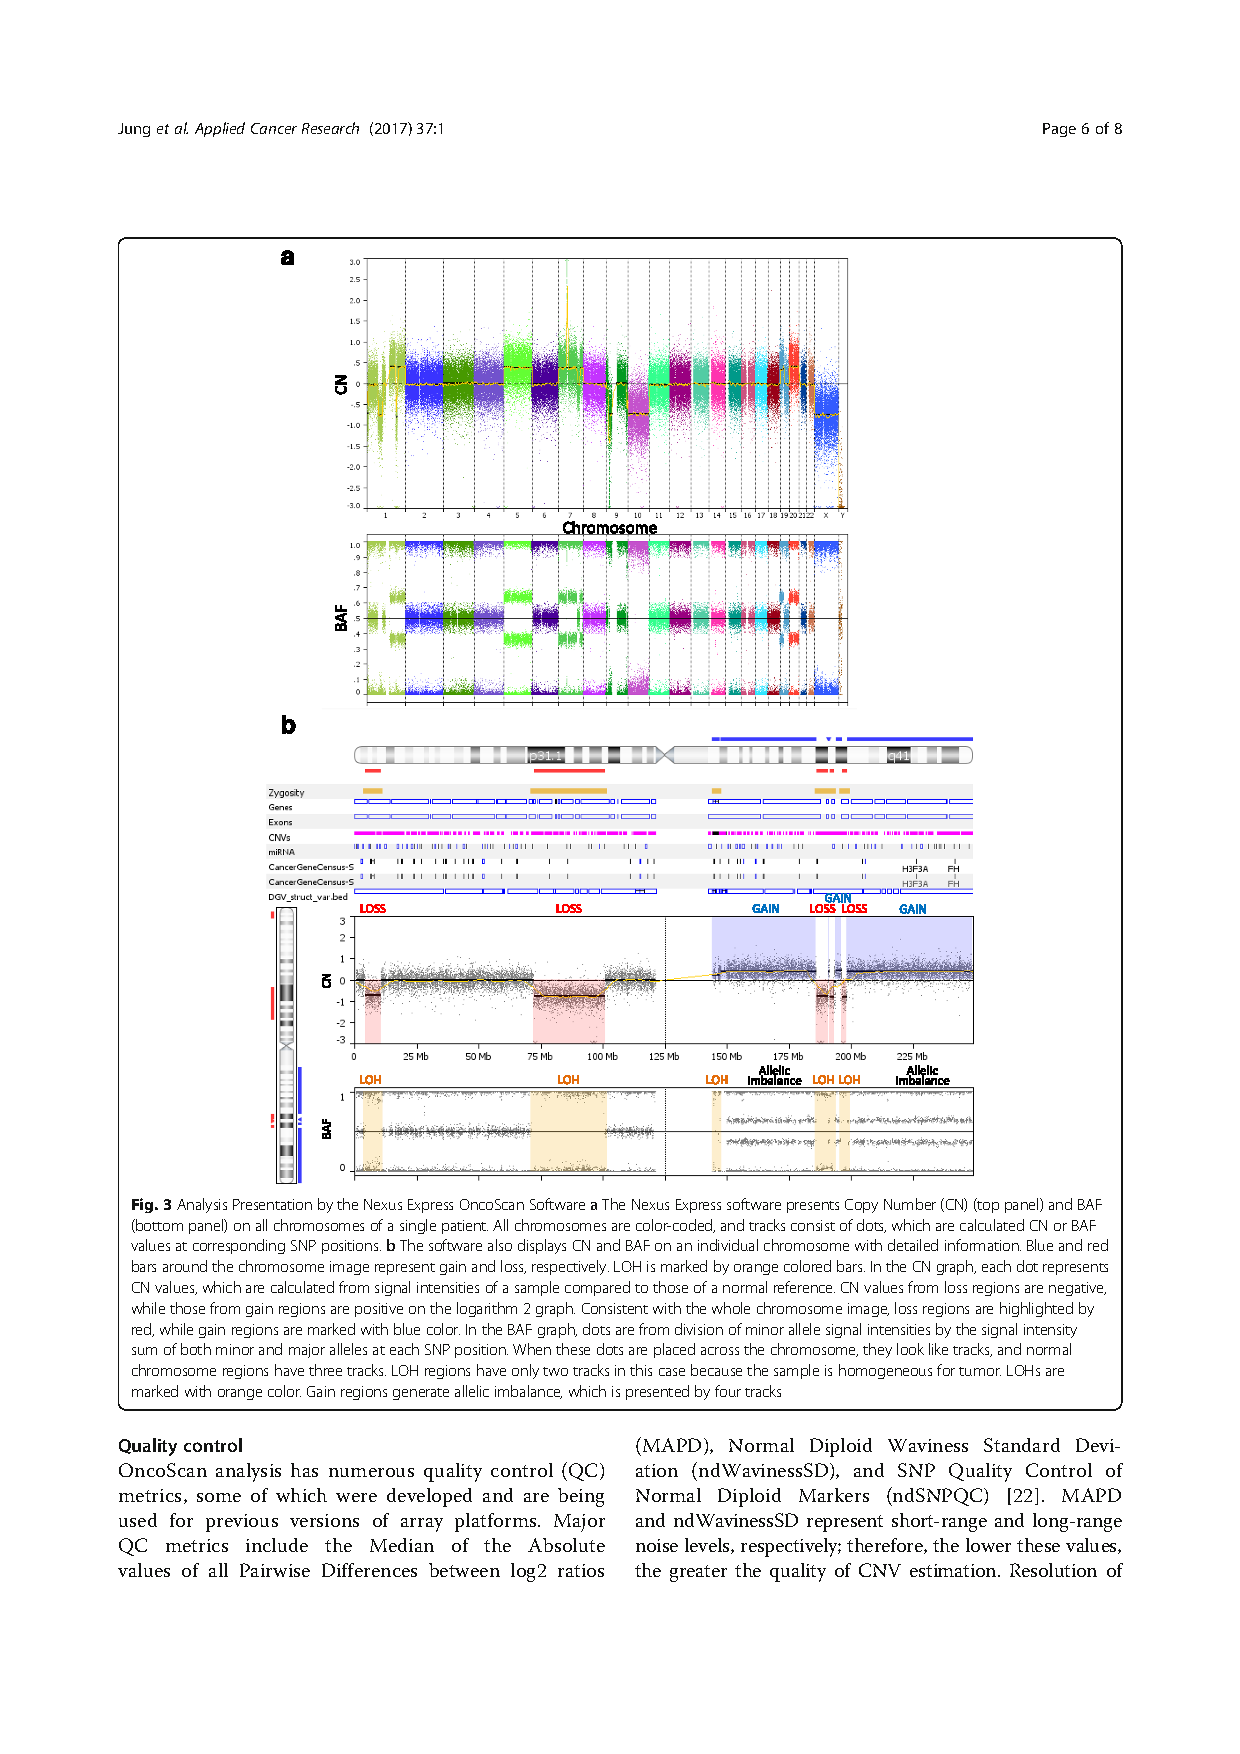
\includegraphics[width=0.9\textwidth, clip,trim=100 268 100 355]{/home/prasad/HUG/Presentation/Oncoscan/oncoscan_assay.pdf}
				\caption{Analysis presentation by the Nexus Express OncoScan Software \footcite {Jung2017,}}
				\label{fig:stream}
				\end{figure}
				\end{frame}	
				
				\subsection{Calculations}
				\begin{frame}
				\begin{mysidebyside}[blanker, lefthand width=.3\linewidth]
				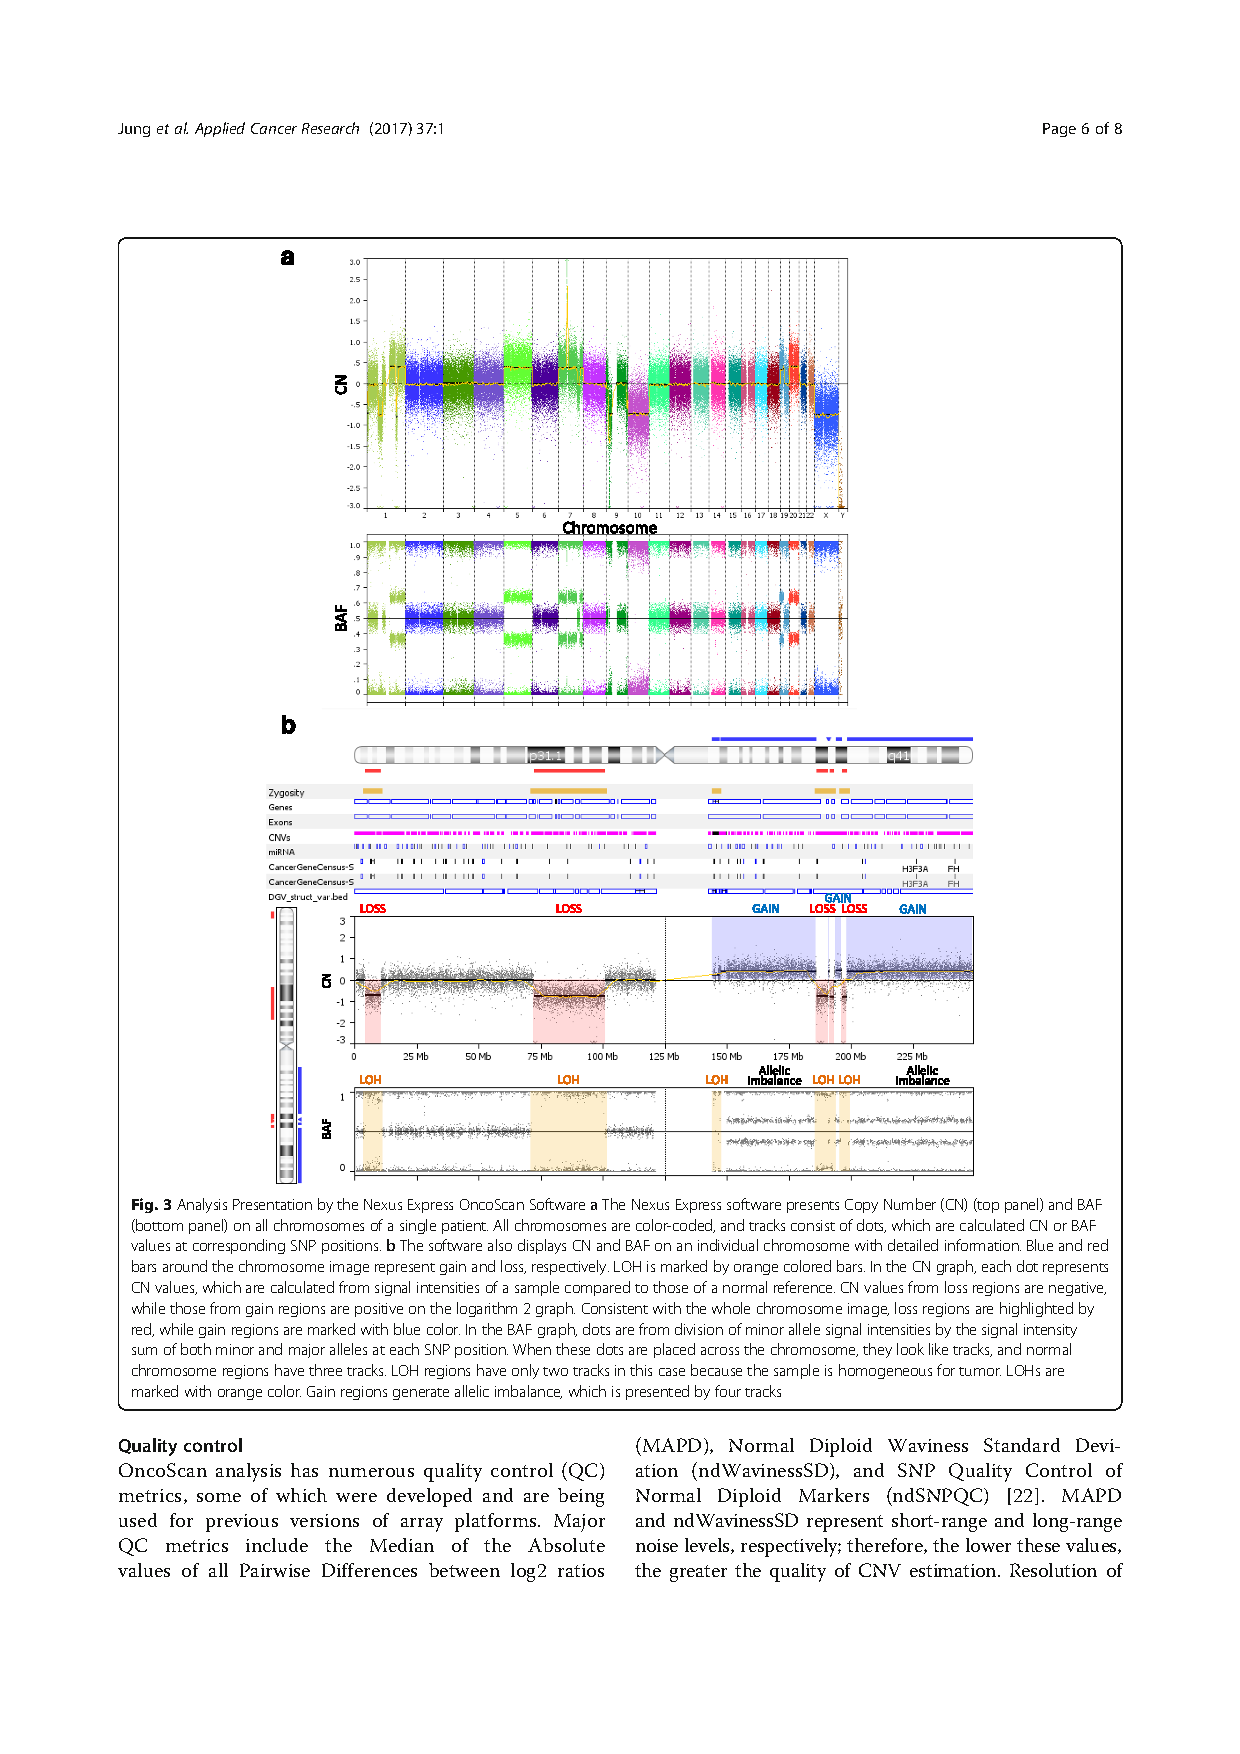
\includegraphics[width=0.6\textwidth, clip,trim=100 270 450 435]{/home/prasad/HUG/Presentation/Oncoscan/oncoscan_assay.pdf}
				\tcblower
				\pause
				\begin{enumerate}
				\item Precise definition of an arm-level alteration
				\pause
				\begin{itemize}								
					\item Percentage of arm to be considered as ``arm-level''?
					\item Contiguity required?
					\item Use of smoothing function?
				\end{itemize}
				\pause
				\item Percentage arm alteration estimation
				\begin{itemize}
				\item Longest segment altered
				\item Sum of all the segments altered 
				\end{itemize}
				\end{enumerate}
				\end{mysidebyside} 
				\end{frame}
	
\section{Results}
                \subsection{Summary}

               \begin{frame}

               \end{frame}

	
\section{Conclusion}
                \subsection{Summary}

               \begin{frame}

               \end{frame}

\section{Acknowledgments}
			\begin{frame}{}
			\huge
			\begin{center}
			Thank You!!!
			\end{center}
			\end{frame}


\end{document}
